% Graph: Análise do número de épocas com desvio padrão no Experimento Gamma
\begin{figure}[H]
	\centering
	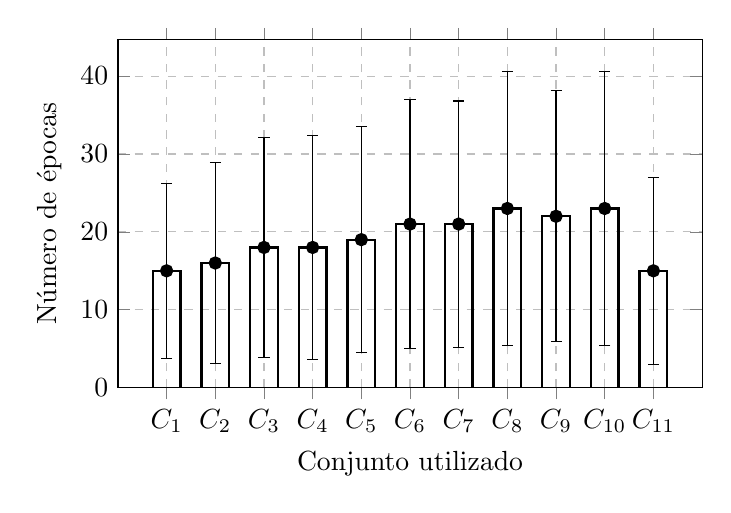
\begin{tikzpicture}
		\begin{axis}[
			% title={Análise do número de épocas com desvio padrão},
			symbolic x coords={$C_1$, $C_2$, $C_3$, $C_4$, $C_5$, $C_6$, $C_7$, $C_8$, $C_9$, $C_{10}$, $C_{11}$},
			xtick={$C_1$, $C_2$, $C_3$, $C_4$, $C_5$, $C_6$, $C_7$, $C_8$, $C_9$, $C_{10}$, $C_{11}$},
			ylabel={Número de épocas},
			xlabel={Conjunto utilizado},
			ybar,
			ymin=0,
			bar width=10pt,
			ymajorgrids=true,
			xmajorgrids=true,
			grid style=dashed,
			height=6cm,
			width=9cm,
		]
		 
		\addplot[color=black, solid, thick, mark=*] plot[error bars/.cd, y dir=both, y explicit]
			coordinates {
				($C_1$,15) +- (28.8,11.2)
				($C_2$,16) +- (19.1,12.9)
				($C_3$,18) +- (21.9,14.1)
				($C_4$,18) +- (21.6,14.4)
				($C_5$,19) +- (23.5,14.5)
				($C_6$,21) +- (26,16)
				($C_7$,21) +- (26.2,15.8)
				($C_8$,23) +- (28.4,17.6)
				($C_9$,22) +- (27.9,16.1)
				($C_{10}$,23) +- (28.4,17.6)
				($C_{11}$,15) +- (18,12)
			}; %\legend{\Bytes}

		\end{axis}
	\end{tikzpicture}
	\caption{Análise do número de épocas com desvio padrão.}
	\label{graph:epochsResultsGamma}
\end{figure}